\documentclass{beamer}
\mode<presentation>
\usepackage{amsmath,amssymb,mathtools}
\usepackage{textcomp}
\usepackage{gensymb}
\usepackage{adjustbox}
\usepackage{subcaption}
\usepackage{enumitem}
\usepackage{multicol}
\usepackage{listings}
\usepackage{url}
\usepackage{graphicx} % <-- needed for images
\def\UrlBreaks{\do\/\do-}

\usetheme{Boadilla}
\usecolortheme{lily}
\setbeamertemplate{footline}{
  \leavevmode%
  \hbox{%
  \begin{beamercolorbox}[wd=\paperwidth,ht=2ex,dp=1ex,right]{author in head/foot}%
    \insertframenumber{} / \inserttotalframenumber\hspace*{2ex}
  \end{beamercolorbox}}%
  \vskip0pt%
}
\setbeamertemplate{navigation symbols}{}

\lstset{
  frame=single,
  breaklines=true,
  columns=fullflexible,
  basicstyle=\ttfamily\tiny   % tiny font so code fits
}

\numberwithin{equation}{section}

% ---- your macros ----
\providecommand{\nCr}[2]{\,^{#1}C_{#2}}
\providecommand{\nPr}[2]{\,^{#1}P_{#2}}
\providecommand{\mbf}{\mathbf}
\providecommand{\pr}[1]{\ensuremath{\Pr\left(#1\right)}}
\providecommand{\qfunc}[1]{\ensuremath{Q\left(#1\right)}}
\providecommand{\sbrak}[1]{\ensuremath{{}\left[#1\right]}}
\providecommand{\lsbrak}[1]{\ensuremath{{}\left[#1\right.}}
\providecommand{\rsbrak}[1]{\ensuremath{\left.#1\right]}}
\providecommand{\brak}[1]{\ensuremath{\left(#1\right)}}
\providecommand{\lbrak}[1]{\ensuremath{\left(#1\right.}}
\providecommand{\rbrak}[1]{\ensuremath{\left.#1\right)}}
\providecommand{\cbrak}[1]{\ensuremath{\left\{#1\right\}}}
\providecommand{\lcbrak}[1]{\ensuremath{\left\{#1\right.}}
\providecommand{\rcbrak}[1]{\ensuremath{\left.#1\right\}}}
\theoremstyle{remark}
\newtheorem{rem}{Remark}
\newcommand{\sgn}{\mathop{\mathrm{sgn}}}
\providecommand{\abs}[1]{\left\vert#1\right\vert}
\providecommand{\res}[1]{\Res\displaylimits_{#1}}
\providecommand{\norm}[1]{\lVert#1\rVert}
\providecommand{\mtx}[1]{\mathbf{#1}}
\providecommand{\mean}[1]{E\left[ #1 \right]}
\providecommand{\fourier}{\overset{\mathcal{F}}{ \rightleftharpoons}}
\providecommand{\system}{\overset{\mathcal{H}}{ \longleftrightarrow}}
\providecommand{\dec}[2]{\ensuremath{\overset{#1}{\underset{#2}{\gtrless}}}}
\newcommand{\myvec}[1]{\ensuremath{\begin{pmatrix}#1\end{pmatrix}}}
\newcommand{\mydet}[1]{\ensuremath{\begin{vmatrix}#1\end{vmatrix}}}
\let\vec\mathbf
% ---------------------

\title{Matgeo Presentation - Problem 2.10.84}
\author{ee25btech11056 - Suraj.N}

\begin{document}

\begin{frame}
  \titlepage
\end{frame}

\begin{frame}{Problem Statement}

Let $Q$ be the cube with the set of vertices 
\[
\{(x_1, x_2, x_3) \mid x_1, x_2, x_3 \in \{0,1\}\} \subset \mathbb{R}^3
\]
Let $F$ be the set of all twelve lines containing the diagonals of the six faces of the cube $Q$.  
Let $S$ be the set of all four lines containing the main diagonals of the cube $Q$; for instance, the line passing through the vertices $(0,0,0)$ and $(1,1,1)$ is in $S$.  

For lines $\lambda_1$ and $\lambda_2$, let $d(\lambda_1, \lambda_2)$ denote the shortest distance between them.  
Then the maximum value of $d(\lambda_1, \lambda_2)$, as $\lambda_1$ varies over $F$ and $\lambda_2$ varies over $S$, is 

\end{frame}

\begin{frame}{Data}

The diagonals of the cube can be written as 

\begin{table}[h!]
  \centering
  \begin{tabular}{|c|c|}
\hline
Line & Equation \\
\hline
Body diagonal & $\vec{x} = \myvec{0\\0\\1} + k_1\myvec{1\\1\\-1}$ \\
\hline
Face diagonal & $\vec{x} = \myvec{0\\0\\0} + k_2\myvec{1\\0\\1}$ \\
\hline
\end{tabular}


  \caption*{Table : diagonals}
  \label{2.10.84}
\end{table}

\end{frame}

\begin{frame}{Solution}

\begin{align}
\vec{x} &= \vec{A} + k_1\vec{m}_1, \quad \vec{A} = \myvec{0\\0\\1}, \; \vec{m}_1 = \myvec{1\\1\\-1} \\
\vec{x} &= \vec{B} + k_2\vec{m}_2, \quad \vec{B} = \myvec{0\\0\\0}, \; \vec{m}_2 = \myvec{1\\0\\1}
\end{align}

\begin{align}
\vec{M} = \myvec{\vec{m_1} & \vec{m_2}} = \myvec{1 & 1 \\1 & 0 \\-1 & 1}
\end{align}

\begin{align}
  \myvec{\vec{B} - \vec{A}} = \myvec{0\\0\\-1}
\end{align}

\end{frame}

\begin{frame}

\begin{align}
\myvec{\vec{M} & \vec{B}-\vec{A}} = \myvec{1 & 1 & 0 \\1 & 0 & 0 \\-1 & 1 & -1}
\end{align}

Performing row operations:
\begin{align}
    \myvec{
        1 & 1 & 0 \\[6pt]
        1 & 0 & 0 \\[6pt]
       -1 & 1 & -1
    }
    &\xleftrightarrow{R_2 \to R_2 - R_1}
    \myvec{
        1 & 1 & 0 \\[6pt]
        0 & -1 & 0 \\[6pt]
       -1 & 1 & -1
    }
    \xleftrightarrow{R_3 \to R_3 + R_1}
    \myvec{
        1 & 1 & 0 \\[6pt]
        0 & -1 & 0 \\[6pt]
        0 & 2 & -1
      }\\
    &\xleftrightarrow{R_3 \to R_3 + 2R_2}
    \myvec{
        1 & 1 & 0 \\[6pt]
        0 & -1 & 0 \\[6pt]
        0 & 0 & -1
    }
\end{align}

Clearly, the rank of this matrix is 3, and therefore, the lines are skew.

\end{frame}

\begin{frame}

From the least squares formulation,  
\begin{align}
  \vec{M}^\top\vec{M}\myvec{k_1 \\ -k_2} &= \vec{M}^\top\myvec{\vec{B}-\vec{A}}
\end{align}

Thus,
\begin{align}
\vec{M}^\top\vec{M} &= 
\myvec{
1 & 1 & -1 \\
1 & 0 & 1
}
\myvec{
1 & 1 \\
1 & 0 \\
-1 & 1
} = \myvec{3 & 0 \\ 0 & 2} \\
\vec{M}^\top(\vec{B}-\vec{A}) &= 
\myvec{1 & 1 & -1 \\ 1 & 0 & 1}
\myvec{0\\0\\-1} 
= \myvec{1 \\ -1}
\end{align}

Therefore,
\begin{align}
\myvec{3 & 0 \\ 0 & 2}
\myvec{k_1 \\ -k_2}
= \myvec{1\\-1}.
\end{align}

\end{frame}

\begin{frame}

Solving,

\begin{align}
  \myvec{k_1\\-k_2} = \myvec{\frac{1}{3} \\[5pt] -\frac{1}{2}}
\end{align}

Hence the closest points are
\begin{align}
\vec{P} &= \vec{A} + k_1\vec{m}_1 
= \myvec{0\\0\\1} + \tfrac{1}{3}\myvec{1\\1\\-1}
= \myvec{\frac{1}{3}\\[5pt] \frac{1}{3}\\[5pt] \frac{2}{3}} \\
\vec{Q} &= \vec{B} + k_2\vec{m}_2 
= \myvec{0\\0\\0} + \tfrac{1}{2}\myvec{1\\0\\1}
= \myvec{\frac{1}{2}\\[5pt] 0\\[5pt] \tfrac{1}{2}}
\end{align}

The shortest distance is
\begin{align}
  \|\vec{P}-\vec{Q}\|
  = \left\|\myvec{-\frac{1}{6}\\[5pt] \tfrac{1}{3}\\[5pt] \tfrac{1}{6}}\right\| = \frac{1}{\sqrt{6}}
\end{align}

 \end{frame}

\begin{frame}{Plot}

\begin{figure}[h!]
  \centering
  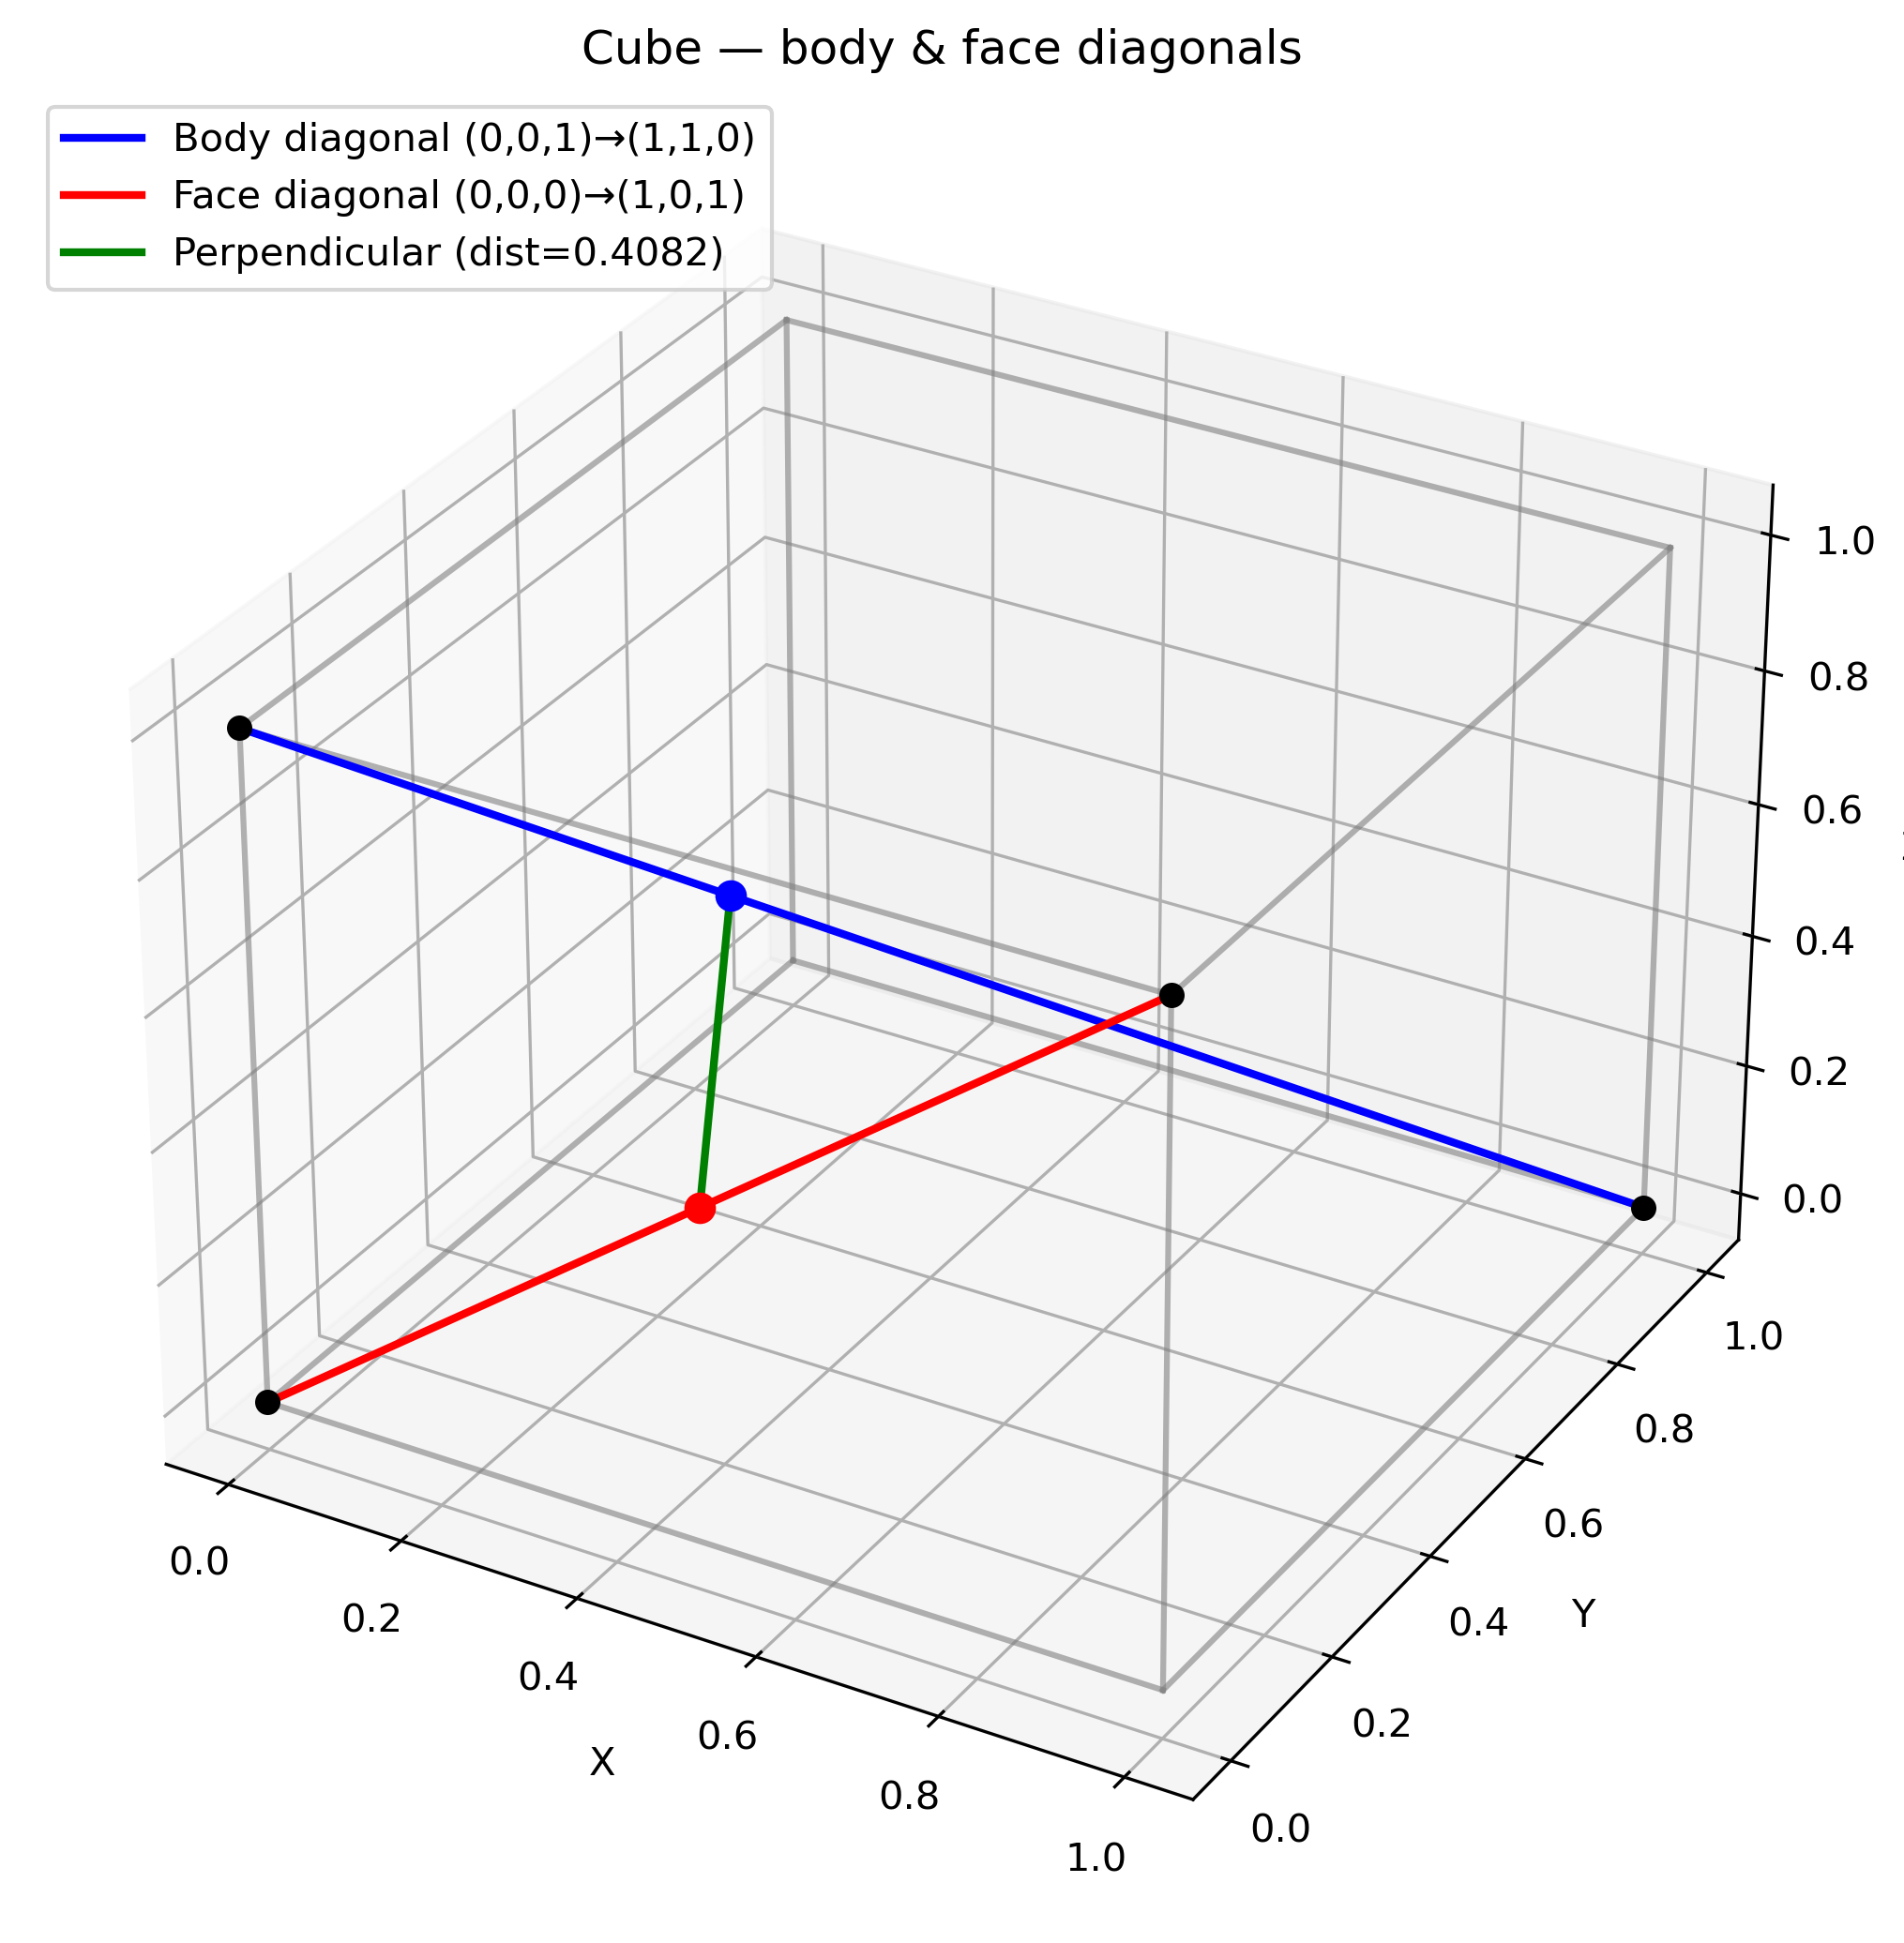
\includegraphics[width=0.6\columnwidth]{figs/cube_lines.png} 
   \caption*{Fig : diagonals}
  \label{Fig1}
\end{figure}
   
\end{frame}

\section*{Appendix: Code}

% C program
\begin{frame}[fragile]{C Code: points.c}
\begin{lstlisting}[language=C]

#include <math.h>
#include <stdio.h>

/* Compute shortest distance between two lines:
   Line1: point P1=(0,0,1), direction d1=(1,1,-1)
   Line2: point P2=(0,0,0), direction d2=(1,0,1)
*/
void compute_distance(double *result) {
  /* Points */
  double p1x = 0.0, p1y = 0.0, p1z = 1.0;
  double p2x = 0.0, p2y = 0.0, p2z = 0.0;

  /* Directions */
  double d1x = 1.0, d1y = 1.0, d1z = -1.0;
  double d2x = 1.0, d2y = 0.0, d2z = 1.0;

  /* P2 - P1 */
  double rx = p2x - p1x;
  double ry = p2y - p1y;
  double rz = p2z - p1z;

  /* cross = d1 x d2 */
  double cx = d1y * d2z - d1z * d2y;
  double cy = d1z * d2x - d1x * d2z;
  double cz = d1x * d2y - d1y * d2x;

  double numer = fabs(rx * cx + ry * cy + rz * cz);
  double denom = sqrt(cx * cx + cy * cy + cz * cz);

  *result = numer / denom;
}

\end{lstlisting}
\end{frame}

% Python calling C
\begin{frame}[fragile]{Python: call\_c.py}
\begin{lstlisting}[language=Python]

# call_c.py
import ctypes
import sys
import numpy as np
import matplotlib.pyplot as plt

# Load C shared lib
lib = ctypes.CDLL("./libpoints.so")
lib.compute_distance.restype = None
lib.compute_distance.argtypes = [ctypes.POINTER(ctypes.c_double)]

# Call C function to get distance
dist = ctypes.c_double()
lib.compute_distance(ctypes.byref(dist))
print("Shortest distance (from C):", dist.value)

# Define endpoints exactly
P1 = np.array([0.0, 0.0, 1.0])    # start of body diagonal
D1 = np.array([1.0, 1.0, -1.0])   # direction -> endpoint P1 + D1 = (1,1,0)
P2 = np.array([0.0, 0.0, 0.0])    # start of face diagonal
D2 = np.array([1.0, 0.0, 1.0])    # direction -> endpoint P2 + D2 = (1,0,1)

# Compute closest points on the two infinite lines (analytic)
w0 = P1 - P2
A = np.dot(D1, D1)
B = np.dot(D1, D2)
C = np.dot(D2, D2)
rhs = np.array([-np.dot(D1, w0), -np.dot(D2, w0)])
M = np.array([[A, -B],[B, -C]])
s, t = np.linalg.solve(M, rhs)   # s for line1, t for line2

\end{lstlisting}
\end{frame}

\begin{frame}[fragile]{Python: call\_c.py}
\begin{lstlisting}[language=Python]


closest1 = P1 + s * D1
closest2 = P2 + t * D2

print("Closest point on body diagonal:", closest1)
print("Closest point on face diagonal:", closest2)
print("Distance between them (computed):", np.linalg.norm(closest1 - closest2))

# --- plotting (neat cube wireframe, diagonals precise, perpendicular segment) ---
def set_axes_equal(ax):
    # make 3D axes equal
    x_limits = ax.get_xlim3d()
    y_limits = ax.get_ylim3d()
    z_limits = ax.get_zlim3d()
    x_range = abs(x_limits[1] - x_limits[0])
    y_range = abs(y_limits[1] - y_limits[0])
    z_range = abs(z_limits[1] - z_limits[0])
    max_range = max(x_range, y_range, z_range)
    x_mid = np.mean(x_limits)
    y_mid = np.mean(y_limits)
    z_mid = np.mean(z_limits)
    half = max_range / 2
    ax.set_xlim(x_mid - half, x_mid + half)
    ax.set_ylim(y_mid - half, y_mid + half)
    ax.set_zlim(z_mid - half, z_mid + half)

fig = plt.figure(figsize=(7,7))
ax = fig.add_subplot(111, projection='3d')

\end{lstlisting}
\end{frame}

\begin{frame}[fragile]{Python: call\_c.py}
\begin{lstlisting}[language=Python]


# cube vertices and edges
vertices = np.array([[0,0,0],[1,0,0],[1,1,0],[0,1,0],
                     [0,0,1],[1,0,1],[1,1,1],[0,1,1]])
edges = [(0,1),(1,2),(2,3),(3,0),
         (4,5),(5,6),(6,7),(7,4),
         (0,4),(1,5),(2,6),(3,7)]
for e in edges:
    a = vertices[e[0]]
    b = vertices[e[1]]
    ax.plot([a[0],b[0]],[a[1],b[1]],[a[2],b[2]], color='gray', alpha=0.6)

# precise diagonals (vertex to vertex lines, no arrows)
ax.plot([P1[0], (P1 + D1)[0] ], [P1[1], (P1 + D1)[1] ], [P1[2], (P1 + D1)[2] ],
        color='blue', linewidth=2, label='Body diagonal (0,0,1)→(1,1,0)')
ax.plot([P2[0], (P2 + D2)[0] ], [P2[1], (P2 + D2)[1] ], [P2[2], (P2 + D2)[2] ],
        color='red', linewidth=2, label='Face diagonal (0,0,0)→(1,0,1)')

# perpendicular shortest segment between the two lines
ax.plot([closest1[0], closest2[0]],
        [closest1[1], closest2[1]],
        [closest1[2], closest2[2]],
        color='green', linewidth=2, label=f'Perpendicular (dist={np.linalg.norm(closest1-closest2):.4f})')

# mark endpoints and closest points
ax.scatter(*(P1), color='black', s=30)
ax.scatter(*((P1 + D1)), color='black', s=30)
ax.scatter(*(P2), color='black', s=30)
ax.scatter(*((P2 + D2)), color='black', s=30)
ax.scatter(*closest1, color='blue', s=50)    # closest on body diag
ax.scatter(*closest2, color='red', s=50)     # closest on face diag

\end{lstlisting}
\end{frame}

\begin{frame}[fragile]{Python: call\_c.py}
\begin{lstlisting}[language=Python]


ax.set_xlabel('X'); ax.set_ylabel('Y'); ax.set_zlabel('Z')
ax.set_title('Cube — body & face diagonals')
ax.legend(loc='upper left')
set_axes_equal(ax)

plt.tight_layout()
plt.savefig("cube_lines.png", dpi=300, bbox_inches='tight')
plt.show()

\end{lstlisting}
\end{frame}

\begin{frame}[fragile]{Python: plot.py}
\begin{lstlisting}[language=Python]
# plot.py
import numpy as np
import matplotlib.pyplot as plt

# Line definitions (exact)
P1 = np.array([0.0, 0.0, 1.0])    # body diagonal start
D1 = np.array([1.0, 1.0, -1.0])   # body diagonal direction -> end (1,1,0)
P2 = np.array([0.0, 0.0, 0.0])    # face diagonal start
D2 = np.array([1.0, 0.0, 1.0])    # face diagonal direction -> end (1,0,1)

# exact shortest distance using cross product
cross = np.cross(D1, D2)
distance = abs(np.dot(P2 - P1, cross)) / np.linalg.norm(cross)
print("Shortest distance (NumPy):", distance)

# compute closest points (solve 2x2 linear system)
w0 = P1 - P2
A = np.dot(D1, D1)
B = np.dot(D1, D2)
C = np.dot(D2, D2)
rhs = np.array([-np.dot(D1, w0), -np.dot(D2, w0)])
M = np.array([[A, -B],[B, -C]])
s, t = np.linalg.solve(M, rhs)
closest1 = P1 + s * D1
closest2 = P2 + t * D2
print("Closest points:", closest1, closest2)
print("Check distance:", np.linalg.norm(closest1 - closest2))

\end{lstlisting}
\end{frame}

\begin{frame}[fragile]{Python: plot.py}
\begin{lstlisting}[language=Python]


# plotting
def set_axes_equal(ax):
    x_limits = ax.get_xlim3d()
    y_limits = ax.get_ylim3d()
    z_limits = ax.get_zlim3d()
    x_range = abs(x_limits[1] - x_limits[0])
    y_range = abs(y_limits[1] - y_limits[0])
    z_range = abs(z_limits[1] - z_limits[0])
    max_range = max(x_range, y_range, z_range)
    x_mid = np.mean(x_limits)
    y_mid = np.mean(y_limits)
    z_mid = np.mean(z_limits)
    half = max_range / 2
    ax.set_xlim(x_mid - half, x_mid + half)
    ax.set_ylim(y_mid - half, y_mid + half)
    ax.set_zlim(z_mid - half, z_mid + half)

fig = plt.figure(figsize=(7,7))
ax = fig.add_subplot(111, projection='3d')

vertices = np.array([[0,0,0],[1,0,0],[1,1,0],[0,1,0],
                     [0,0,1],[1,0,1],[1,1,1],[0,1,1]])
edges = [(0,1),(1,2),(2,3),(3,0),
         (4,5),(5,6),(6,7),(7,4),
         (0,4),(1,5),(2,6),(3,7)]
for e in edges:
    a = vertices[e[0]]
    b = vertices[e[1]]
    ax.plot([a[0],b[0]],[a[1],b[1]],[a[2],b[2]], color='gray', alpha=0.6)

\end{lstlisting}
\end{frame}

\begin{frame}[fragile]{Python: plot.py}
\begin{lstlisting}[language=Python]

# diagonals as precise lines from vertex to vertex (no arrowheads)
ax.plot([P1[0], P1[0]+D1[0]],[P1[1], P1[1]+D1[1]],[P1[2], P1[2]+D1[2]],
        color='blue', linewidth=2, label='Body diagonal (0,0,1)→(1,1,0)')
ax.plot([P2[0], P2[0]+D2[0]],[P2[1], P2[1]+D2[1]],[P2[2], P2[2]+D2[2]],
        color='red', linewidth=2, label='Face diagonal (0,0,0)→(1,0,1)')

# exact perpendicular segment
ax.plot([closest1[0], closest2[0]],
        [closest1[1], closest2[1]],
        [closest1[2], closest2[2]],
        color='green', linewidth=2, label=f'Perpendicular (dist={distance:.4f})')

# markers for vertices and closest points
ax.scatter(*P1, color='black', s=30)
ax.scatter(*(P1 + D1), color='black', s=30)
ax.scatter(*P2, color='black', s=30)
ax.scatter(*(P2 + D2), color='black', s=30)
ax.scatter(*closest1, color='blue', s=50)
ax.scatter(*closest2, color='red', s=50)

ax.set_xlabel('X'); ax.set_ylabel('Y'); ax.set_zlabel('Z')
ax.set_title('Cube — body & face diagonals')
ax.legend(loc='upper left')
set_axes_equal(ax)

plt.tight_layout()
plt.savefig("cube_lines.png", dpi=300, bbox_inches='tight')
plt.show()



\end{lstlisting}
\end{frame}




\end{document}
